\documentclass[tikz,convert={density=300,size=300x300,outfile=\jobname.png}]{standalone}

\usetikzlibrary{automata,calc,trees,positioning,arrows,chains,shapes.geometric,%
decorations.pathreplacing,decorations.pathmorphing,shapes,%
matrix,shapes.symbols,plotmarks,decorations.markings,shadows}

\begin{document}


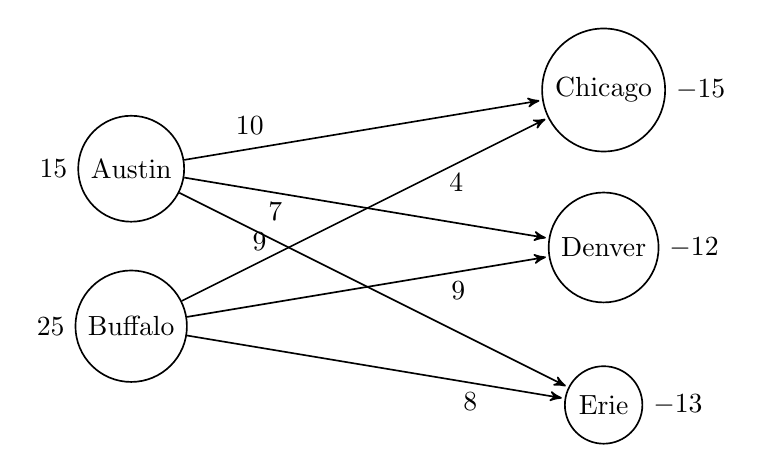
\begin{tikzpicture}[->,>=stealth',shorten >=1pt,auto,node distance=2.8cm,
                    semithick]

  \node[state] at(1,5) (node1) [label=left:15] {Austin};
  \node[state] at(1,3) (node2) [label=left:25] {Buffalo};
  \node[state] at(7,6) (node3) [label=right:$-15$] {Chicago};
  \node[state] at(7,4) (node4) [label=right:$-12$] {Denver};
  \node[state] at(7,2) (node5) [label=right:$-13$] {Erie};

  \path (node1) edge node [near start]{10} (node3)
        (node1) edge node [near start, below]{7} (node4)
        (node1) edge node [near start, left]{9} (node5)
        (node2) edge node [near end, below]{4} (node3)
        (node2) edge node [near end, below]{9} (node4)
        (node2) edge node [near end, below]{8} (node5)
        ;

\end{tikzpicture}

\end{document}